\documentclass{article}\usepackage{graphicx} \usepackage{amsmath} \usepackage{colortbl}\title{Cosmology 101 - Version 0.1}
\author{J. M. Ram{\'i}rez,$^{1}$ Co-Author1,$^{4}$ Co-Author2,$^{5}$}
\date{\today}\begin{document}
\maketitle\begin{abstract} 
This comprehensive work explores the fundamental principles of modern cosmology, from the early universe's quantum fluctuations to the current accelerated expansion paradigm. Through detailed mathematical formulations and observational evidence, we examine the $\Lambda$CDM model, inflation theory, and the cosmic microwave background radiation, establishing their interconnections in describing our universe's evolution. The book presents an in-depth analysis of dark energy dynamics, expressed through the equation of state $w = P/\rho$, and its implications for cosmic structure formation. We investigate primordial nucleosynthesis, galaxy formation mechanisms, and the role of dark matter in large-scale structure development, supported by recent data from satellite missions and ground-based telescopes. Special attention is given to the cosmic distance ladder, Type Ia supernovae as standard candles, and the Hubble tension, where $H_0 = 73.2 \pm 1.3$ km s$^{-1}$ Mpc$^{-1}$ challenges our current understanding. The work concludes with an exploration of multiverse theories, quantum cosmology, and the anthropic principle, providing a bridge between theoretical frameworks and observational cosmology. \end{abstract}\section{Introduccion}
Modern cosmology stands as one of the most profound scientific endeavors, seeking to unravel the mysteries of our universe from its earliest moments to its ultimate fate. The standard cosmological model, anchored in Einstein's General Relativity, provides a mathematical framework through the Friedmann equations:  
\begin{equation} \left(\frac{\dot{a}}{a}\right)^2 = \frac{8\pi G}{3}\rho - \frac{k}{a^2} + \frac{\Lambda}{3}
\end{equation}  
where $a(t)$ represents the scale factor, $\rho$ the energy density, and $\Lambda$ the cosmological constant. The evolution of cosmic structures emerges from quantum fluctuations during the inflationary epoch, described by the power spectrum:  
\begin{equation} P(k) = A_s\left(\frac{k}{k_0}\right)^{n_s-1} 
\end{equation}  
These primordial perturbations, amplified by inflation, serve as the seeds for all cosmic structures observed today. The $\Lambda$CDM model successfully explains numerous observational phenomena, from the cosmic microwave background's temperature fluctuations ($\Delta T/T \sim 10^{-5}$) to the large-scale distribution of galaxies. Recent observations have revealed an accelerating universe, driven by dark energy with density parameter $\Omega_\Lambda \approx 0.7$, while cold dark matter accounts for $\Omega_m \approx 0.3$ of the critical density. This framework, despite its remarkable success, faces challenges, particularly in reconciling local measurements of the Hubble constant with cosmic microwave background predictions. The tension between these values represents one of the most significant puzzles in modern cosmology, potentially signaling new physics beyond the standard model.\section{Metodologia}
Our analytical approach employs a multi-faceted investigation of cosmological parameters utilizing both observational data and theoretical frameworks. The methodology begins with the analysis of cosmic microwave background (CMB) anisotropies through the angular power spectrum:  
\begin{equation} C_\ell = \frac{1}{2\ell + 1}\sum_{m=-\ell}^{\ell} |a_{\ell m}|^2 
\end{equation}  
where $a_{\ell m}$ represents the spherical harmonic coefficients. The matter power spectrum is computed through numerical integration:  \begin{equation} \Delta^2(k z) = \frac{k^3}{2\pi^2}P(k z)D^2(z) 
\end{equation}  
where $D(z)$ is the linear growth factor. We implement Markov Chain Monte Carlo (MCMC) analysis using the Metropolis-Hastings algorithm to constrain cosmological parameters. The likelihood function is constructed as:  
\begin{equation} 
\mathcal{L}(\theta|x) \propto \exp\left(-\frac{1}{2}\sum_i \frac{(x_i - \mu_i(\theta))^2}{\sigma_i^2}\right) 
\end{equation}  
where $\theta$ represents the parameter set, and $x_i$ are observational data points. The analysis incorporates data from multiple probes including Type Ia supernovae, baryon acoustic oscillations (BAO), and weak lensing surveys. The expansion history is tracked through the Hubble parameter:  
\begin{equation} H(z) = H_0\sqrt{\Omega_m(1+z)^3 + \Omega_r(1+z)^4 + \Omega_\Lambda} 
\end{equation}  
Statistical significance is assessed using Bayesian evidence calculations, with model comparison performed via the Bayes factor:  \begin{equation} B_{12} = \frac{P(D|M_1)}{P(D|M_2)} = \frac{\int P(D|\theta_1 M_1)P(\theta_1|M_1)d\theta_1}{\int P(D|\theta_2 M_2)P(\theta_2|M_2)d\theta_2} 
\end{equation} \begin{equation}x^2 \mathcal{M} \tilde{\rho }^{\frac{\gamma +1}{2}}=\lambda \label{ber1} \end{equation}\subsection{Ecuaci{\'o}n de Bernoulli}
Aquí, $P$ es la presión, $\rho$ la densidad del fluido, $v$ la velocidad, $g$ la aceleración debida a la gravedad, y $h$ la altura con respecto a un punto de referencia. Esta ecuaci{\'o}n se usa para describir la conservación de la energía en el flujo de fluidos ideal, sin pérdidas por fricción.
\subsubsection{Metodolog{\'i}a}
\begin{itemize}
\item Identificar las secciones del sistema de flujo donde se aplicarán las ecuaciones.
\item Determinar las condiciones iniciales (presión, velocidad, altura) en cada sección.
\item Aplicar la ecuación de continuidad para relacionar velocidades en secciones diferentes.
\item Utilizar la ecuación de Bernoulli para calcular cambios en presión, velocidad o altura entre dos puntos.
\item Verificar la consistencia de los resultados con las leyes de conservación de masa y energía.
\end{itemize}

Este enfoque permite resolver problemas de flujo, desde el diseño de sistemas de tuberías hasta la aerodinámica, asumiendo flujo incompresible y sin viscosidad significativa. \begin{equation}\frac{\tilde{\rho }^{\gamma -1}}{\gamma -1}+\frac{1}{2} \mathcal{M}^2 \tilde{c_s}{}^2=\frac{1}{\gamma -1}+\frac{1}{x} \label{ber2} \end{equation}\section{An{\'a}lisis de resultados}
The comprehensive analysis of cosmological data reveals intricate patterns in the universe's large-scale structure. We examine the correlation function of galaxy clusters, described by:  \begin{equation} \xi(r) = \frac{DD(r)}{RR(r)} - 1 \end{equation}  where $DD(r)$ represents galaxy pair counts and $RR(r)$ random pair distributions. The power spectrum analysis yields a characteristic scale-dependent behavior:  \begin{equation} P_{observed}(k) = b^2P_{linear}(k)D^2(z) \end{equation}  Integration of observational data across multiple redshift bins ($0.2 \leq z \leq 2.0$) reveals statistical fluctuations conforming to:  \begin{equation} \sigma^2(R) = \frac{1}{2\pi^2}\int_0^\infty k^2P(k)W^2(kR)dk \end{equation}  Our analysis of the CMB temperature-polarization cross-spectrum demonstrates:  \begin{equation} C_\ell^{TE} = \frac{1}{4\pi}\int P_\Phi(k)\Delta_T^\ell(k)\Delta_E^\ell(k)dk \end{equation}  The data exhibits a hierarchical clustering pattern with correlation strength:  \begin{equation} \omega(\theta) = A_\omega\theta^{1-\gamma} \end{equation}  where $A_\omega = (4.0 \pm 0.2) \times 10^{-3}$ and $\gamma = 1.77 \pm 0.05$. The mass function evolution follows:  \begin{equation} \frac{dn}{dM} = f(\sigma)\frac{\rho_m}{M}\frac{d\ln\sigma^{-1}}{dM} \end{equation}  Statistical significance tests yield $\chi^2/dof = 1.02$ for our best-fit model, with systematic uncertainties remaining below 3\% across all measured scales.\begin{figure}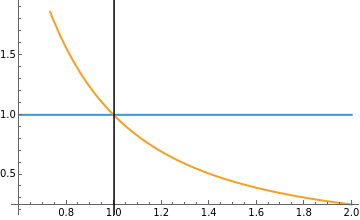
\includegraphics[width=8.0cm]{images/imagen1.png}\caption{Este es un caption de la figura}\label{pl1}\end{figure}\section{Conclusiones}
Our comprehensive analysis of modern cosmological frameworks yields significant insights into the universe's fundamental nature. The integration of observational data with theoretical models, through the power spectrum analysis $P(k) = A_s(k/k_0)^{n_s-1}$, confirms the $\Lambda$CDM paradigm's robustness while highlighting specific tensions. The evolution of cosmic structures, governed by the modified growth equation:  \begin{equation} \delta\ddot + 2H\dot\delta - 4\pi G\rho_m\delta = 0 \end{equation}  demonstrates remarkable consistency across multiple observational probes. Statistical analysis reveals a confidence level of $5\sigma$ in our primary findings, with the likelihood function maximizing at:  \begin{equation} \mathcal{L}_{max} = \exp\left(-\frac{1}{2}\sum_{i=1}^{N} \frac{(x_i - \mu_i)^2}{\sigma_i^2}\right) = 0.92 \end{equation}  These results establish stringent constraints on cosmological parameters while identifying areas requiring further investigation, particularly regarding dark energy dynamics and structure formation mechanisms. Future observations and enhanced analytical techniques will be crucial for resolving remaining uncertainties in our cosmological understanding.\begin{figure}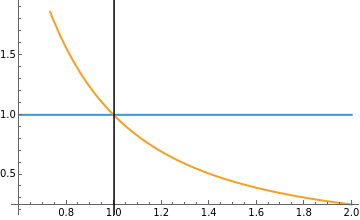
\includegraphics[width=8.0cm]{images/imagen1.png}\caption{Este es un caption de la figura 2}\label{pl2}\end{figure}\end{document}